
%(BEGIN_QUESTION)
% Copyright 2010, Tony R. Kuphaldt, released under the Creative Commons Attribution License (v 1.0)
% This means you may do almost anything with this work of mine, so long as you give me proper credit

This is a pressure alarm circuit, designed to energize a warning light if the process pressure sensed by the pressure switch ever crosses a certain threshold value:

$$\includegraphics[width=15.5cm]{i02004x01.eps}$$

First, determine if this is a {\it low-pressure} alarm or a {\it high-pressure alarm} (i.e. under what type of process pressure condition will the light bulb energize, an abnormally low pressure or an abnormally high pressure?).

\vskip 20pt

Next, determine the effect of a bad wire connection (``open'' fault) at terminal 2 of the control relay on the status of the warning light.

\vfil 

\underbar{file i02004}
\eject
%(END_QUESTION)





%(BEGIN_ANSWER)

This is a graded question -- no answers or hints given!

%(END_ANSWER)





%(BEGIN_NOTES)

This is a {\bf low-pressure} alarm circuit.

\vskip 10pt

The consequence of this wiring fault is that the warning light will {\bf always be on}.

%INDEX% Pictorial circuit review (relay circuit)

%(END_NOTES)


